\chapter{Analyse}

\section{Logoot}
	\emph{logoot} est un algorithme destiné à l'édition de documents textes sur
	un réseau \emph{pair-à-pair} (cf. \ref{sec:p2p}). Concrètement, cet
	algorithme permet de partager la position des caractères du document entre
	les différentes personnes travaillant dessus.
	
	\subsection{Principe de fonctionnement}
		Chaque utilisateur possède un tableau dans lequel y est placé la
		position de tous les caractères du document collaboratif. Ces derniers
		sont identifié par un identifiant unique appelé \emph{identifiant de
		caractère}. Lorsqu'un caractère est ajouté par un utilisateur, ce
		dernier est envoyé à travers le réseau afin que tous les autres
		utilisateurs puissent mettre à jour	son	tableau et le document.\\
		
		Initialement, l'algorithme \emph{Logoot} est basé sur des identifiants
		de position de ligne. Cependant, dans un travail collaboratif, une même
		ligne peut être modifiée en même temps par plusieurs personnes
		(répliques), il est	donc nécessaire de non plus avoir un identifiant par
		ligne mais bien par caractère. Un \emph{identifiant de position} est
		un triplet
		\verb+<i,s,h>+ avec 
		\begin{itemize}
			\item \emph{i} : un chiffre dans la base \emph{BASE}. La valeur
			maximum que peut prendre \emph{i} \emph{MAX} sera entre $0$ et
			\emph{BASE}$ - 1$.
			\item \emph{s} : un identifiant unique de la réplique.
			\item \emph{h} : la valeur de l'horloge logique de la réplique.
		\end{itemize}~
		
		Un \emph{identifiant de caractère} est une liste ordonnée non-mutable d'
		\emph{identifiants de positions}. Voici un exemple d'\emph{identifiant
		de caractère}: \\
		\verb+<42, 1, 1><1337, 1, 72>+ ou encore \verb+<2, 4, 4>+\\
		
		La \emph{table des identifiants} permet de stocker les identifiants de
		caractères ce qui permet, via une recherche dichotomique, d'acceder à
		tous les caractères du document.
		
	\subsection{Insertion dans le document}
	
		Pour insérer un nouveau caractère, il faut calculer son identifiant afin
		que les autres utilisateurs sachent où le placer dans le document. La
		table \ref{tab:tableID}	p.\pageref{tab:tableID} est la table d'origine
		d'un document qui est:
		\verb+ab+.\\
		\begin{table}
			\center
			\begin{tabular}{|l|l|l|}			
			\hline
				Table des identifiants & Identifiant de caractère & Caractère\\
			\hline
				0 & \verb+<0, NA, NA>+ & NA\\
				1 & \verb+<41, 3, 1>+ & a\\
				2 & \verb+<44, 2, 16>+ & b\\
				MAX & \verb+<MAX, NA, NA>+ & NA\\
			\hline
			\end{tabular}
			\caption{Exemple de table des identifiants - Origine}
			\label{tab:tableID}
		\end{table}
		
		L'explication de l'insertion se fera par l'exemple, on veut ajouter deux
		caractères 'c' et 'd' entre les lettres 'a' et 'b' qui ont pour
		identifiants \verb+<41, 3, 1>+ et \verb+<44, 2, 16>+.
		\begin{enumerate}
			\item Les identifiants des caractères des éléments précédent et
			suivant sont récupérés (via la table des identifiants):
			\verb+<prefPrev, sPrev, hPrev>+ et \verb+<prefNext, sNext, hNext>+
			\item On regarde si on a la <<place>> pour placer les nouveaux
			identifiants\\ \verb+interval = prefNext - prefPrev - 1;+ ce qui
			donne\\ \verb+interval = 44 - 41 - 1 = 2;+. Il y a donc la place
			pour générer deux identifiants de taille un (c'est-à-dire un seul
			triplet	par	identifiant de caractère).
			\item Les identifiants sont générés dans l'interval disponible, on a
			donc: \verb+<42, 1, 1>+ et \verb+<43, 1, 2>+
			La table \ref{tab:tableID_cd} p.\pageref{tab:tableID_cd} représente
			la table des identifiants après l'ajout des deux lettres.
				
		\begin{table}
			\center
			\begin{tabular}{|l|l|l|}			
			\hline
				Table des identifiants & Identifiant de caractère & Caractère\\
			\hline
				0 & \verb+<0, NA, NA>+ & NA\\
				1 & \verb+<41, 3, 1>+ & a\\
				2 & \verb+<42, 1, 1>+ & c\\
				3 & \verb+<43, 1, 2>+ & d\\
				4 & \verb+<44, 2, 16>+ & b\\
				MAX & \verb+<MAX, NA, NA>+ & NA\\
			\hline
			\end{tabular}
			\caption{Exemple de table des identifiants - Insertion de 'c' et
			'd'}
			\label{tab:tableID_cd}
		\end{table}
			\item Le Document mis a jour est:
				\verb+acdb+
		\end{enumerate}~
		
		On veut maintenant ajouter le caractère 'e' entre 'c' et 'd'.
		\begin{enumerate}
			\item Les identifiants des caractères des éléments précédent et
			suivant sont récupérés (via la table des identifiants):
			\verb+<prefPrev, sPrev, hPrev>+ et \verb+<prefNext, sNext, hNext>+
			\item On regarde si on a la <<place>> pour placer le nouvel
			identifiant\\ \verb+interval = prefNext - prefPrev - 1;+ ce qui
			donne \\
			\verb+interval = 43 - 42 - 1 = 0;+. Il n'y a pas de place, le
			nouvel identifiant sera donc préfixé par \verb+<42, 1, 1>+.
			\item Afin de calculer le nouvel identifiant \emph{i}, on determine
			l'interval de choix de \emph{i} qui sera entre le précédent et le
			suivant concaténé avec le triplet minimum:\\
			\verb+<42, 1, 1><0, 1, x>+\\ 
			\verb+<43, 1, 2><0, 1, x>+\\
			Nous avons donc un interval de \emph{MAX} positions disponibles.
			\item ]0, MAX[ est donc l'interval dans lequel sera généré le
			\emph{i} suivant:\\
			\verb+<42, 1, 1><5, 1, 3>+\\
			Le choix de \emph{i} dans l'interval est réalisé par un algorithme
			de génération (cf. \ref{sec:algos}).
			La table \ref{tab:tableID_e} p.\pageref{tab:tableID_e} représente la
			table des identifiants après l'ajout des deux lettres.
				
		\begin{table}
			\center
			\begin{tabular}{|l|l|l|}			
			\hline
				Table des identifiants & Identifiant de caractère & Caractère\\
			\hline
				0 & \verb+<0, NA, NA>+ & NA\\
				1 & \verb+<41, 3, 1>+ & a\\
				2 & \verb+<42, 1, 1>+ & c\\
				3 & \verb+<42, 1, 1><5, 1, 3>+ & e\\
				4 & \verb+<43, 1, 2>+ & d\\
				5 & \verb+<44, 2, 16>+ & b\\
				MAX & \verb+<MAX, NA, NA>+ & NA\\
			\hline
			\end{tabular}
			\caption{Exemple de table des identifiants - Insertion de 'e'}
			\label{tab:tableID_e}
		\end{table} 
		\end{enumerate}~
		
		\subsubsection{Algorithme de génération des
		identifiants}\label{sec:algos}
		Il existe deux algorithmes qui permettent de générer les identifiants:
		\emph{Random} et \emph{Boundary}.\\
		
		\textbf{Random:}\\
			Les identifiants sont générés aléatoirement parmi tous ceux de
			l'interval.\\
		
		\textbf{Boundary:}\\
			Comme pour le \emph{random}, les identifiants sont générés
			aléatoirement mais deux identifiants successifs ne peuvent espacés
			de plus d'une valeur notée \emph{boundary}. Cette stratégie permet
			de laisser un plus grand interval pour les insertions futures car on
			prend en compte le fait que les insertions ont généralement lieu en
			fin de document qu'au début.
		
	\subsection{Suppression dans le document}
		
		Pour supprimer un élément, son \emph{identifiant de caractère} est tout
		simplement supprimé de la table des identifiants.
		
\section{Pair-à-Pair}\label{sec:p2p}

	Un réseau pair-à-pair est un modèle ou chaque client est aussi serveur. En
	effet, dans un réseau pair-à-pair, l'information est diffusée au travers du
	réseau grâce aux clients qui relaient l'information. Comme représenté en
	figure \ref{fig:p2p} page \pageref{fig:p2p}, le réseau est décentralisé,
	chaque ordinateur joue un double rôle de client et de serveur. L'avantage
	d'un tel réseau est qu'il soit décentralisé, en effet, la vie d'une
	ressource ne repose pas sur un seul serveur (comme c'est le cas dans un
	réseau classique) mais bien sûr tous les éléments du réseau qui la possède.
	Ainsi, même si l'un des noeuds cesse d'émettre, la ressource reste
	disponible via les autres noeuds qui la possède.
	
	\begin{figure}
	  \center
      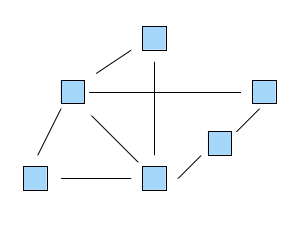
\includegraphics[width=0.4\textwidth]{includes/P2P-network.png}
      \caption{Exemple de réseau pair-à-pair}
      \label{fig:p2p}
    \end{figure}
	
	\subsection{Gossip}
	
		Gossip est un protocole de communication basé sur l'idée
		d'\emph{épidémie} ou de rumeur: une personne lance une rumeur à ses
		voisins qui eux-même la disent à leurs voisins, etc au bout d'un certain
		temps, toutes personnes connaissent la rumeur lancée par une celle
		d'origine.
		
		L'avantage d'utiliser \emph{Gossip} est qu'il permet de fonctionner dans
		un réseau non structuré. En effet, en utilisant \emph{Gossip}, il n'est
		pas nécessaire de connaitre la structure du réseau pour pouvoir
		fonctionner.
		
		On suppose que l'on souhaite faire la recherche d'un ressource X qui se
		trouve sur l'un des postes du réseau, le principe du protocole est le
		suivant:
		\begin{enumerate}
			\item Chaque noeud possède une liste de \emph{peer} dans le réseau.
			\item À intervale régulier, le poste prend un peer au hazard dans la
			liste et lui envoie le message.
			\item Le poste qui reçoit le message vérifie s'il possède la
			ressource: si c'est le cas, il répond, sinon il recommence depuis
			l'étape 2 et ainsi de suite.
		\end{enumerate}~
		De cette façon, en un temps logarithmique, chaque noeud du réseau aura
		reçu le message et l'initiateur de la recherche aura donc la réponse. À
		chaque "tour", le nombre de personne renvoyant le message est doublé ce
		qui rend le protocole très robuste car, même si un message est perdu en
		cours de route, le noeud qui aura manqué ce message, le recevra de la
		part d'un autre peer.\\
		
		Ce protocole est la solution pour le projet. En effet, le réseau sur
		lequel les personnes font le travail collaboratif n'est pas connu et
		encore moins structuré. Une implémentation java est disponible par
		l'Inria, cependant lors de la recherche d'un protocole peer-to-peer, ce
		dernier était encore en cours de développement ce qui rendait son
		utilisation très difficile, de plus, la pauvreté de documentation
		concernant le code ne facilitait pas la tâche d'apprentissage. C'est
		pour cela que nous n'avons pas retenu \emph{Gossip} pour le réseau
		peer-to-peer
	
	\subsection{Jxta}
		JXTA est une technologie open source permettant de faire un réseau
		pair-à-pair en Java. Le principe est simple, un réseau pair-à-pair est
		créé sur le réseau existant permettant aux différents noeuds de pouvoir
		communiquer entre eux.\\
		
		Étant un projet connu, la communauté derrière cette technologie et
		l'abondante documentation ont permis de choisir et d'utiliser
		\emph{Jxta} assez facilement.